\chapter{Top-Down Parsing: Psycholinguistic Adequacy}
\label{cha:TopDownEval}

\section{Two Basic Advantages}
\label{sec:TopDownEval_Advantages}

\subsection{Incrementality}
\label{sub:TopDownEval_Incrementality}
The most basic requirement for a psychologically plausible parser is that it works in an incremental fashion, that is to say, parsing can take place as soon as the first word of the sentence has been uttered, rather than delaying parsing until the full sentence has been heard.
You showed in an earlier exercise that the top-down parser only needs to keep track of the starting position of an item, which entails that it can be run in an incremental fashion.

\subsection{Simplicity}
\label{sub:TopDownEval_Simplicity}
Top-down parsers are conceptually simple.
The top-down orientation of the parser mirrors the view of CFGs as top-down generators.
In addition, the inference rules are extremely simple (compared to, say, \emph{left-corner parsing}, which we will discuss at a later point), seeing how the inference rule of the parser directly mirrors the rewrite rules of the grammar.
This is particularly appealing for proponents of a \emph{transparent parser}.
A transparent parser must use the grammar in as direct a fashion as possible.
That precludes processing-based explanations of syntactic phenomena --- e.g.\ island effects --- and prioritizes a maximally simple parser. 

\section{Garden Path Effects}
\label{sec:TopDownEval_GardenPath}

\subsection{Garden Paths as Backtracking}
\label{sub:TopDownEval_Frazier}
One of the best known phenomena in syntactic processing are \emph{garden path effects}, which arise with sentences that are grammatically well-formed but nonetheless difficult to parse \citep{Frazier79, FrazierRayner82}.
More precisely, a garden path sentence is a sentence $w$ that up to some $w_i$ has a strongly preferred analysis that must be discarded at $w_{i+1}$. 
Here's a list of examples that includes more than the usual suspects:
%
\begin{exe}
    \ex \emph{Structural ambiguity}
    \begin{xlist}
        \ex The horse raced past the barn fell.
        \ex The raft floated down the river sank.
        \ex The player tossed a Frisbee smiled.
        \ex The doctor sent for the patient arrived.
        \ex The cotton clothing is made of grows in Mississippi.
        \ex Fat people eat accumulates.
        \ex I convinced her children are noisy.
    \end{xlist}
    %
    \ex \emph{Lexical ambiguity}
    \begin{xlist}
        \ex The old train the young.
        \ex The old man the boat.
        \ex Until the police arrest the drug dealers control the street.
        \ex The dog that I had really loved bones.
        \ex The man who hunts ducks out on weekends.
    \end{xlist}
\end{exe}

\citet{Frazier79} proposes to treat garden path effects as a result of reanalysis: the parser is forced to abandon its current set of hypotheses, backtrack to an earlier point, and build a new structure from there.
If for some reason this process proves too difficult, the parser gets stuck and assigns no structure at all.

This kind of analysis is compatible with top-down parsing, depending on the data structure we use.
Remember that the data structure keeps track of the items in the current parse, but also of alternative parses.
The control structure includes a set of instructions for which parses should be prioritized.
Let's try to make \possciteauthor{Frazier79} account precise using a top-down parser with priority queues as data structure and a serial strategy for expanding multiple parses.

\subsection{Priority Queues and Prefix Trees}
\label{sub:TopDownEval_PriorityQueues}
Let's assume that our data structure is a \emph{priority queue}, i.e.\ a list of parse tables that can be reordered, to which we can add new entries, and from which we can delete old entries (note: even though I call it a list, that doesn't mean queues are best implemented as lists; in Python, for example, you're better off using arrays).

As so often, a more abstract perspective is helpful here.
Instead of a list of parse tables, we can use a \emph{prefix tree} as a unified way of representing multiple parses at once.
The root of the prefix tree is always our start axiom [0,S] (since the final position is redundant for top-down parsing, it can be safely omitted).
If parse item $q$ is obtained from item $p$ via a prediction or scan rule, $q$ is added to the tree as a daughter of $p$.
Furthermore, each node that is not a leaf is also subscripted with the list of unused predict rules. 
We call a node in this tree a \emph{parse leaf} iff it is a leaf or has at least one subscript, and a (strictly descending) path spanning from the root to a leaf or a parse leaf is called a \emph{parse path}.
The set of parse tables, then, corresponds exactly to the set of parse paths.
Putting all of this together, we can implement a priority queue as a ranking of parse paths through the prefix tree.
%
\begin{examplebox}{Parse Tables as Trees}
Suppose we are using the grammar from the beginning of Lecture~\ref{cha:TopDown} to parse \emph{the anvil hit Daffy} with a recursive descent parser.
Our parse table starts with [0,\psep S] as usual, from which we can only predict [0,\psep NP VP].
This can be represented as the tree below.
%
\begin{center}
    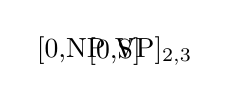
\begin{tikzpicture}
        \Tree
            [.\node(root){[0,\psep S]};
                \node (0) {[0,\psep NP VP]$_{2,3}$};
            ]
    \end{tikzpicture}
\end{center}
%
Note that [0,\psep NP VP] has subscripts $2$ and $3$ to indicate that we can use rules 2 and 3 of our CFG to predict new parse items.
Suppose the parser uses predict(3) to create the item [0,\psep Det N VP].
Then this item is added as a daughter of [0,\psep NP VP] to the previous tree, and the subscript 3 is also removed from [0,\psep NP VP].
We do not need to add a subscript to [0,\psep Det N VP] since it is a leaf.
%
\begin{center}
    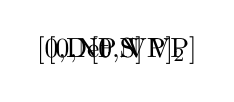
\begin{tikzpicture}
        \Tree
            [.\node(root){[0,\psep S]};
                [.\node(0){[0,\psep NP VP]$_{2}$};
                    \node(00){[0,\psep Det N VP]};
                ]
            ]
    \end{tikzpicture}
\end{center}
%
The next step of the parser now depends on how the control structure prioritizes distinct parses.
We can either expand the table that ends in [0,\psep Det N VP], or go back to the one ending in [0,\psep NP VP] and apply predict(2).
Suppose we do the latter, so that [0,\psep PN VP] is added as the second daughter of [0,\psep NP VP], which thus loses its last subscript.
%
\begin{center}
    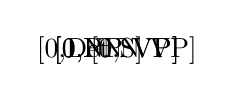
\begin{tikzpicture}
        \Tree
            [.\node(root){[0,\psep S]};
                [.\node(0){[0,\psep NP VP]};
                    \node(00){[0,\psep Det N VP]};
                    \node(01){[0,\psep PN VP]};
                ]
            ]
    \end{tikzpicture}
\end{center}
%
Now let's expand [0,\psep Det N VP] again to obtain [0, \psep the N VP] and then apply a scan step, yielding [1, \psep N VP].
%
\begin{center}
    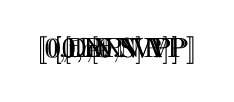
\begin{tikzpicture}
        \Tree
            [.\node(root){[0,S]};
                [.\node(0){[0,NP VP]};
                    [.\node(00){[0,Det N VP]};
                        [.\node(000){[0,the N VP]};
                            \node (0000) {[1,N VP]};
                        ]
                    ]
                    \node(01){[0,PN VP]};
                ]
            ]
    \end{tikzpicture}
\end{center}
%
If our parser is really smart, it will be able to infer at this point that the scanned word \emph{the} can never be obtained from [0,PN VP] (technically this is achieved by associating every parse item $p$ with a regular expression that describes the possible left edges of the strings that can be derived from $p$).
So the parser can remove [0,PN VP] from the tree, which is tantamount to discarding the parse table where NP was rewritten as PN\@.
%
\begin{center}
    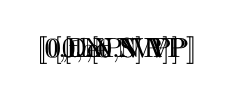
\begin{tikzpicture}
        \Tree
            [.\node(root){[0,S]};
                [.\node(0){[0,NP VP]};
                    [.\node(00){[0,Det N VP]};
                        [.\node(000){[0,the N VP]};
                            \node (0000) {[1,N VP]};
                        ]
                    ]
                ]
            ]
    \end{tikzpicture}
\end{center}

\end{examplebox}

What makes the tree representation of parse tables appealing is that the construction and prioritization of parse tables can be reduced to strategies for tree building.
In particular, the familiar notions of depth-first and breadth-first carry over in a natural fashion.
%
\begin{description}
    \item[depth first/serial] expand a parse item $p$ that was introduced during the previous parse step; if the parse item $p$ cannot be expanded, expand the lowest parse leaf $l$ that dominates $p$
    \item[breadth first/parallel] before expanding a parse item introduced during parse step $j$, all parse items that were introduced at parsing step $i$ must have been rewritten, for every $i < j$
\end{description}
%
The depth first strategy leads to a parser that always builds a single complete parse history rather than multiple partial ones.
If the parse history cannot be expanded anymore, the parser either stops (successful parse) or backtracks to the last choice point in the parse history and tries a different choice instead.
This corresponds exactly to the notion of \emph{serial parsing} in the psycholinguistic literature.

The intuitive counterpart of serial parsing is \emph{fully parallel parsing}, where all parse tables are built up at the same time.
This is exactly the behavior of the breadth-first strategy.
However, even proponents of parallel parsing usually do not assume that the human parser computes and stores all options all the time.
Instead, only a subset of very likely parses is claimed to be worked on in parallel, with all others either discarded or at least not expanded on.
On a technical level we may formalize this in terms of a probabilistic procedure for which parse items may be expanded, and in which order.
The details are not important here, the basic insights is simply that just as we can add probabilities to the control schema to regulate which inference rules the parser may apply, we can also use probabilities to prioritize the expansion of certain parse tables over others.

\subsection{Formal Account of Garden Paths}
\label{sub:TopDownEval_FormalGardenPath}
A recursive descent parser with a depth-first expansion strategy for prefix trees, coupled with a preference ranking over prediction steps, can easily account for garden path effects.
In the case of \emph{the horse raced past the barn fell}, for example, the parse builds a single parse table, and due to how certain rewrite rules are preferred over others, this parse table encodes the structure for \emph{the horse raced past the barn}.
When encountering \emph{fell}, the parser has to backtrack.
A successful parse requires backtracking to the point where \emph{raced} is analyzed as part of the VP rather than the NP --- that's quite a distance.
%
\begin{examplebox}[Backtracking in \emph{the horse raced past the barn fell}]
    Assume we have the following (massively simplified) grammar:
    %
    \begin{center}
        \begin{tabular}{rrlp{2em}rrl}
            1)  & S   & \rewrite NP VP
                & & 
            8)  & Det & \rewrite the
            \\
            2)  & NP  & \rewrite Det N
                & &
            9)  & N   & \rewrite barn
            \\
            3)  & NP  & \rewrite Det N VP$_\mathit{rel}$
                & & 
            10) & N   & \rewrite horse 
            \\
            4)  & VP  & \rewrite V
                & & 
            11) & P   & \rewrite past
            \\
            5)  & VP  & \rewrite V PP
                & & 
            12) & V   & \rewrite fell 
            \\
            6)  & VP$_\mathit{rel}$  & \rewrite V$_\mathit{rel}$ PP
                & & 
            13) & V   & \rewrite raced
            \\
            7)  & PP  & \rewrite P NP
                & & 
            14) & V$_\mathit{rel}$   & \rewrite raced
        \end{tabular}
    \end{center}
    %
    Here's the resulting tree for our garden path sentence.
    %
    \begin{center}
        \begin{tikzpicture}
            \Tree
                [.S
                    [.NP
                        [.Det the ]
                        [.N horse ]
                        [.VP$_\mathit{rel}$
                            [.V$_\mathit{rel}$ raced ]
                            [.PP
                                [.P past ]
                                [.NP
                                    [.Det the ]
                                    [.N barn ]
                                ]
                            ]
                        ]
                    ]
                    [.VP
                        [.V fell ]
                    ]
                ]
        \end{tikzpicture}
    \end{center}
    %
    If the parser prefers NP \rewrite\ Det N over NP \rewrite Det N CP and operates in a recursive descent fashion, the construction of the first parse table results in the prefix tree below.
    %
    \begin{center}
        \footnotesize
        \begin{tikzpicture}[level 1+/.style = { level distance = 2em }]
            \Tree
                [.{[0,\psep S]}
                [.{[0,\psep NP VP]$_3$}
                [.{[0,\psep Det N VP]}
                [.{[0, \psep the N VP]}
                [.{[1,\psep N VP]$_9$}
                [.{[1,\psep horse VP]}
                [.{[2,\psep VP]$_4$}
                [.{[2,\psep V PP]$_{12}$}
                [.{[2,\psep raced PP]}
                [.{[3,\psep PP]}
                [.{[3,\psep P NP]}
                [.{[3,\psep past NP]}
                [.{[4,\psep NP]$_3$}
                [.{[4,\psep Det N]}
                [.{[4,\psep the N]}
                [.{[5,\psep N]$_{10}$}
                [.{[5,\psep barn]}
                [.{[6,\psep]}
                ]]]]]]]]]]]]]]]]]]
        \end{tikzpicture}
    \end{center}
    %
    Since this parse does not succeed, the parser needs to backtrack.
    The closest choice point is [5,\psep N]$_{10}$, which obviously does not fix the problem of integrating \emph{fell} into the structure, as can be verified after a single scan step.
    The next choice point is [4,\psep NP]$_3$.
    Here the parser still has the option of replacing NP by Det N CP, which won't help much either, but it takes quite a while to realize this because the tree for the parse table obtained by following this option involves a choice point, too.
    %
    \begin{center}
        \footnotesize
        \begin{tikzpicture}[level 1+/.style = { level distance = 2em }]
            \Tree
                [.{[4,\psep NP]}
                    [.{[4,\psep Det N VP$_\mathit{rel}$]}
                        [.{[4,\psep the N VP$_\mathit{rel}$]}
                            [.{[5,\psep N VP$_\mathit{rel}$]}
                                [.{[5,\psep barn VP$_\mathit{rel}$]}
                                    [.{[6,\psep VP$_\mathit{rel}$]}
                                        [.{[6,\psep V$_\mathit{rel}$ PP]}
                                            {[6,\psep fell PP]}
                                        ]
                                    ]
                                ]
                                {[5,\psep horse VP$_\mathit{rel}$]}
                            ]
                        ]
                    ]
                ]
        \end{tikzpicture}
    \end{center}
    %
    Since this venue didn't yield a successful parse either, the parse backtracks to [2,\psep V PP]$_{12}$, and after this fails, to [2,\psep VP]$_4$.
    Once again it is not successful, and the same holds once it expands [1,\psep N VP].
    %
    \begin{center}
        \footnotesize
        \begin{tikzpicture}[level 1+/.style = { level distance = 2em }]
            \Tree
                [.{[2,\psep V PP]}
                    {[2,\psep fell PP]}
                ]

            \begin{scope}[xshift=8em]
                \Tree
                    [.{[2,\psep VP]}
                        [.{[2,\psep V]}
                            {[2,\psep fell]}
                            {[2,\psep raced]}
                        ]
                    ]
            \end{scope}

            \begin{scope}[xshift=16em]
                \Tree
                    [.{[1,\psep N VP]}
                        {[1,\psep barn VP]}
                    ]
            \end{scope}
        \end{tikzpicture}
    \end{center}
    %
    Only if the parser backtracks all the way to [0,\psep NP VP]$_3$, essentially undoing all its work so far, can it find a working parse.
    %
    \begin{center}
        \footnotesize
        \begin{tikzpicture}[level 1+/.style = { level distance = 2em}]
            \Tree
                [.{[0,\psep NP VP]}
                    [.{[0,\psep Det N VP$_\mathit{rel}$ VP]}
                        [.{[0,\psep the N VP$_\mathit{rel}$ VP]}
                            [.{[1,\psep N VP$_\mathit{rel}$ VP]}
                                {[1,\psep barn VP$_\mathit{rel}$ VP]}
                                [.{[1,\psep horse VP$_\mathit{rel}$ VP]}
                                    [.{[2,\psep VP$_\mathit{rel}$ VP]}
                                        [.{[2,\psep V$_\mathit{rel}$ PP VP]}
                                            [.{[3,\psep raced PP VP]}
                                                [.{[4,\psep PP VP]}
                                                    [.{[4,\psep P NP VP]}
                                                        [.{[4,\psep past NP VP]}
                                                            [.{[5,\psep NP VP]}
                                                                [.{[5,\psep Det N VP]}
                                                                    [.{[5,\psep the N VP]}
                                                                        [.{[6,\psep N VP]$_{10}$}
                                                                            [.{[6,\psep barn VP]}
                                                                                [.{[7,\psep VP]}
                                                                                    [.{[7,\psep V]$_{13}$}
                                                                                        [.{[7,\psep fell]}
                                                                                            {[7,\psep]}
                                                                                        ]
                                                                                    ]
                                                                                ]
                                                                            ]
                                                                        ]
                                                                    ]
                                                                ]
                                                            ]
                                                        ]
                                                    ]
                                                ]
                                            ]
                                        ]
                                    ]
                                ]
                            ]
                        ]
                    ]
                ]
        \end{tikzpicture}
    \end{center}
    %
    The prefix tree for all the parse histories built by the parser before it encounters a successful parse it much bigger than the simple phrase structure tree for the sentence.
    %
    \begin{center}
        \footnotesize
        \begin{tikzpicture}[%
            level 1+/.style = { level distance = 2em },
            level 5/.style = { sibling distance= -5em },
            level 7/.style = { sibling distance= -5em },
            level 8/.style = { sibling distance= -10em }
            ]
            \Tree
                [.{[0,\psep S]}
                    [.{[0,\psep NP VP]}
                        [.{[0,\psep Det N VP]}
                            [.{[0, \psep the N VP]}
                                [.{[1,\psep N VP]}
                                    [.{[1,\psep horse VP]}
                                        [.{[2,\psep VP]}
                                            [.{[2,\psep V PP]}
                                                [.{[2,\psep raced PP]}
                                                    [.{[3,\psep PP]}
                                                        [.{[3,\psep P NP]}
                                                            [.{[3,\psep past NP]}
                                                                [.{[4,\psep NP]}
                                                                    [.{[4,\psep Det N]}
                                                                        [.{[4,\psep the N]}
                                                                            [.{[5,\psep N]}
                                                                                [.{[5,\psep barn]}
                                                                                    {[6,\psep]}
                                                                                ]
                                                                                {[5,\psep horse]}
                                                                            ]
                                                                        ]
                                                                    ]
                                                                    [.{[4,\psep Det N VP$_\mathit{rel}$]}
                                                                        [.{[4,\psep the N VP$_\mathit{rel}$]}
                                                                            [.{[5,\psep N VP$_\mathit{rel}$]}
                                                                                [.{[5,\psep barn VP$_\mathit{rel}$]}
                                                                                    [.{[6,\psep VP$_\mathit{rel}$]}
                                                                                        [.{[6,\psep V$_\mathit{rel}$ PP]}
                                                                                            {[6,\psep fell PP]}
                                                                                        ]
                                                                                    ]
                                                                                ]
                                                                                {[5,\psep horse VP$_\mathit{rel}$]}
                                                                            ]
                                                                        ]
                                                                    ]
                                                                ]
                                                            ]
                                                        ]
                                                    ]
                                                ]
                                                {[2,\psep fell PP]}
                                            ]
                                            [.{[2,\psep V]}
                                                {[2,\psep raced]}
                                                {[2,\psep fell]}
                                            ]
                                        ]
                                    ]
                                {[1,\psep barn VP]}
                                ]
                            ]
                        ]
                        [.{[0,\psep Det N VP$_\mathit{rel}$ VP]}
                            [.{[0,\psep the N VP$_\mathit{rel}$ VP]}
                                [.{[1,\psep N VP$_\mathit{rel}$ VP]}
                                    {[1,\psep barn VP$_\mathit{rel}$ VP]}
                                    [.{[1,\psep horse VP$_\mathit{rel}$ VP]}
                                        [.{[2,\psep VP$_\mathit{rel}$ VP]}
                                            [.{[2,\psep V$_\mathit{rel}$ PP VP]}
                                                [.{[3,\psep raced PP VP]}
                                                    [.{[4,\psep PP VP]}
                                                        [.{[4,\psep P NP VP]}
                                                            [.{[4,\psep past NP VP]}
                                                                [.{[5,\psep NP VP]}
                                                                    [.{[5,\psep Det N VP]}
                                                                        [.{[5,\psep the N VP]}
                                                                            [.{[6,\psep N VP]$_{10}$}
                                                                                [.{[6,\psep barn VP]}
                                                                                    [.{[7,\psep VP]}
                                                                                        [.{[7,\psep V]$_{13}$}
                                                                                            [.{[7,\psep fell]}
                                                                                                {[7,\psep]}
                                                                                            ]
                                                                                        ]
                                                                                    ]
                                                                                ]
                                                                            ]
                                                                        ]
                                                                    ]
                                                                ]
                                                            ]
                                                        ]
                                                    ]
                                                ]
                                            ]
                                        ]
                                    ]
                                ]
                            ]
                        ]
                    ]
                ]
        \end{tikzpicture}
    \end{center}
\end{examplebox}

\subsection{Center Embedding}
\label{sub:TopDownEval_CenterEmbedding}
It is a well-known fact that center embedding constructions are harder to parse than right embedding constructions, even if one controls for sentence length, discourse and vocabulary.
%
\begin{exe}
    \ex
    \begin{xlist}
        \ex I bought the cheese (that) the mouse (that) the cat (that) the dog chased ate wanted.
        \ex I bought the cheese (that) the mouse wanted (that) the cat ate (that) the dog wanted.
    \end{xlist}
\end{exe}
%
A common idea is that the difficulty of center embedding has to do with an increased memory burden, either because more items have to be kept in memory for a non-trivial amount of time, or because specific items have to be stored for a longer time, or a combination of the two.
The specifics vary between accounts.

\citet{Kimball73}, for instance, proposes that the parser cannot work on more than two sentences at once, i.e.\ it is possible to keep up to two CPs in memory, but not more than that.
Right embedding of CPs is fine because opening a new CP is the last step needed to close the containing CP, which can subsequently be removed from memory.
Center embedding, on the other hand, requires that both CPs be stored in memory, so it is natural limited to one level of embedding.

\posscitet{Gibson98} \emph{Syntactic Prediction Locality Theory} (SPLT) contends that memory burden increases the more dependencies need to be stored at the same time, and since center embedding of the type NP-S-VP necessarily involves starting a new dependency before the old one between NP and VP has been finished, center embedding is difficult.

This argument can be ported into our more formal setting via a \emph{linking hypothesis} between control structure and processing difficulty.
Remember that we can annotate phrase structure trees to indicate the order in which nodes are introduced and rewritten by the parser.
Obviously any item that is not rewritten immediately after its introduction --- i.e.\ any item whose prefix and suffix differ by more than 1 --- needs to be stored in memory.
Let's put these items in boxes so that they are easy to pick out at a glance.
Parsing difficulty, then, can be measured in a variety of ways.
%
\begin{description}
    \item[Tenure] the \emph{tenure of node $n$} is the difference between its subscript and its superscript
    \item[Payload] the \emph{payload of tree $t$} is the number of nodes whose tenure is strictly greater than $1$
\end{description}
%
These two measures can be combined to create a variety of difficulty metrics such as the two below (cf.\ \citealt{Kobele.etal12} and \citealt{GrafMarcinek14CMCL}).
%
\begin{description}
    \item[MaxTen] greatest tenure among all the nodes; $\max(\setof{ \mathrm{tenure}(n) })$
    \item[SumTen] total number of steps that items must be memorized; $\sum(\setof{ \mathrm{tenure}(n) > 1})$
\end{description}
%
All of these metrics capture the fact that right embedding isn't harder than center embedding.
\textbf{MaxTen} and \textbf{SumTen} also predict right embedding to be easier.

\begin{examplebox}[Center embedding and maximum tenure]
    Consider the center embedding and right embedding trees below, which have been annotated according to the behavior of a recursive descent parser.
    For center embedding we are using a promotion-style analysis of relative clauses \citep{Vergnaud74, Kayne94}, which posits that the relative clause is an argument of the determiner, with the head noun residing in a CP specifier.
    For right embedding the extraposed relative clause is considered a daughter of S.
    %
    \begin{center}
        \footnotesize
        \begin{tikzpicture}[
            level 1+/.style = { level distance = 2.5em },
            level 2/.style = { sibling distance = -.75em },
            level 3/.style = { sibling distance = -1em },
            level 4/.style = { sibling distance = -1em },
            level 5/.style = { sibling distance = -2.5em }
            ]
            \Tree
                [.\Lab{S}{1}{2}
                    [.\Lab{NP}{2}{3}
                        [.\Lab{N}{3}{4}
                            \Lab{I}{4}{5}
                        ]
                    ]
                    [.\IBLab{VP}{2}{6}
                        [.\Lab{V}{6}{7}
                            \Lab{bought}{7}{8}
                        ]
                        [.\IBLab{NP}{6}{9}
                            [.\Lab{Det}{9}{10}
                                \Lab{the}{10}{11}
                            ]
                            [.\IBLab{CP}{9}{12}
                                [.\Lab{N}{12}{13}
                                    \Lab{cheese}{13}{14}
                                ]
                                [.\IBLab{C}{12}{15}
                                    \Lab{that}{15}{16}
                                ]
                                [.\IBLab{S}{12}{17}
                                    [.\Lab{NP}{17}{18}
                                        [.\Lab{Det}{18}{19}
                                            \Lab{the}{19}{20}
                                        ]
                                        [.\IBLab{CP}{18}{21}
                                            [.\Lab{N}{21}{22}
                                                \Lab{mouse}{22}{23}
                                            ]
                                            [.\IBLab{C}{21}{24}
                                                \Lab{that}{24}{25}
                                            ]
                                            [.\IBLab{S}{21}{26}
                                                [.\Lab{NP}{26}{27}
                                                    [.\Lab{Det}{27}{28}
                                                        \Lab{the}{28}{29}
                                                    ]
                                                    [.\IBLab{N}{27}{30}
                                                        \Lab{cat}{30}{31}
                                                    ]
                                                ]
                                                [.\IBLab{VP}{26}{32}
                                                    [.\Lab{V}{32}{33}
                                                        \Lab{ate}{33}{34}
                                                    ]
                                                ]
                                            ]
                                        ]
                                    ]
                                    [.\IBLab{VP}{17}{34}
                                        [.\Lab{V}{34}{35}
                                            \Lab{wanted}{35}{36}
                                        ]
                                    ]
                                ]
                            ]
                        ]
                    ]
                ]
        \end{tikzpicture}

        \begin{tikzpicture}[
            level 1+/.style = { level distance = 2.5em },
            level 2/.style = { sibling distance = -.75em },
            level 3/.style = { sibling distance = -1em },
            level 4/.style = { sibling distance = -1em },
            level 5/.style = { sibling distance = -1em },
            level 6/.style = { sibling distance = -1em }
            ]
            \Tree
                [.\Lab{S}{1}{2}
                    [.\Lab{NP}{2}{3}
                        [.\Lab{N}{3}{4}
                            \Lab{I}{4}{5}
                        ]
                    ]
                    [.\IBLab{VP}{2}{6}
                        [.\Lab{V}{6}{7}
                            \Lab{bought}{7}{8}
                        ]
                        [.\IBLab{NP}{6}{9}
                            [.\Lab{Det}{9}{10}
                                \Lab{the}{10}{11}
                            ]
                            [.\IBLab{CP}{9}{12}
                                [.\Lab{N}{12}{13}
                                    \Lab{cheese}{13}{14}
                                ]
                                [.\IBLab{C}{12}{15}
                                    \Lab{that}{15}{16}
                                ]
                                [.\IBLab{S}{12}{17}
                                    [.\Lab{NP}{17}{18}
                                        [.\Lab{Det}{18}{19}
                                            \Lab{the}{19}{20}
                                        ]
                                        [.\IBLab{N}{18}{21}
                                            \Lab{mouse}{21}{22}
                                        ]
                                    ]
                                    [.\IBLab{VP}{17}{23}
                                        [.\Lab{V}{23}{24}
                                            \Lab{wanted}{24}{25}
                                        ]
                                    ]
                                    [.\IBLab{CP}{17}{26}
                                        [.\Lab{C}{27}{28}
                                            \Lab{that}{28}{29}
                                        ]
                                        [.\IBLab{S}{27}{30}
                                            [.\Lab{NP}{30}{31}
                                                [.\Lab{Det}{31}{32}
                                                    \Lab{the}{32}{33}
                                                ]
                                                [.\IBLab{N}{31}{34}
                                                    \Lab{cat}{34}{35}
                                                ]
                                            ]
                                            [.\IBLab{VP}{30}{36}
                                                [.\Lab{V}{36}{37}
                                                    \Lab{ate}{37}{38}
                                                ]
                                            ]
                                        ]
                                    ]
                                ]
                            ]
                        ]
                    ]
                ]
        \end{tikzpicture}
    \end{center}
    %
    The difficult center embedding sentence has a payload of 11, a maximum tenure of 17, and a sum tenure of 55.
    The easier right embedding sentence has a payload of 11, a maximum tenure of 9, and a sum tenure of 48.
    Irrespective of how we weigh or rank these three metrics, then, right embedding is never predicted to be harder than center embedding.
    As long as we do not take payload as the only difficulty metric, right embedding is correctly predicted to be easier than center embedding.
\end{examplebox}

Notice that our explanation for the difficulty of center embedding is very different from the one we used for garden path effects.
Garden path effects were explained in terms of the difficulty of finding a right parse among the many possible ones.
We used prefix trees as a way of representing the parser's route through this search space, and since a prefix tree encodes many parsing tables at ones, our account is ultimately based on the processing challenges of coordinating multiple parse tables --- if all parse tables could be easily stored in memory and expanded in a breadth-first manner, garden path effects would not arise.

Center embedding, on the other hand, is explained purely in terms of how the parser constructs the correct parse.
How the parser actually finds this parse does not factor into the explanation.
The claim is that even if the parser had a perfect \emph{oracle}, a machine that could tell it at every step which inference step must be taken to get the correct structure, the difference between center embedding and right embedding would not disappear because the former still puts a higher load on working memory than the latter.

\section{Problems}
\label{sec:TopDownEval_Problems}

\subsection{Memory Usage in Left Embedding}
\label{sub:TopDownEval_LeftEmbedding}
A careful examination of the top-down parsers behavior over center embedding constructions reveals that these configurations aren't the only ones that should cause an increased memory burden.
Coupled with our metrics of processing difficulty, a recursive descent parser predicts that left embedding should be hard to parse, too --- which is not borne out empirically.
%
\begin{exe}
    \ex
    \begin{xlist}
        \ex The exhaust pipe of the car of the father of the mechanic is broken.
        \ex The mechanic's father's car's exhaust pipe is broken.
    \end{xlist}
\end{exe}
%
The cause for the predicted difficulty spike with left embedding is straight-forward.
Suppose the parser conjectures at step $i$ that node $n$ in the tree has daughters $d_1$ and $d_2$.
Steps $i+1$ to $j$ are spent by the parser expanding the subtree rooted in $d_1$.
The bigger the subtree, the higher the value of $j + 1$, the point at which the parser can move on to expanding $d_2$.
Since $d_2$ must be kept in memory from step $i$ until step $j + 1$, and the value of $j$ increases with the size of the subtree rooted in $d_1$, every construction that increases the size of a left sibling --- including left embedding --- should increase parsing difficulty.

\subsection{Looping in Left Recursion}
\label{sub:TopDownEval_LeftRecursion}

Left embedding constructions are problematic for top-down parsers in more respects than just psycholinguistic adequacy.
Consider a grammar that licenses possessive structures such as the one below.
%
\begin{center}
    \begin{tikzpicture}
        \Tree
            [.S
                [.NP
                    [.NP
                        [.NP
                            [.N John ]
                        ]
                        [.Poss 's ]
                        [.N father ]
                    ]
                    [.Poss 's ]
                    [.N car ]
                ]
                [.VP
                    [.V disappeared ]
                ]
            ]
    \end{tikzpicture}
\end{center}
%
In order to arrive at this structure, the parser must first infer [0,\psep NP VP], and then expand the NP to get [0,\psep NP Poss N VP].
But now the parser once again has to expand the NP, possibly creating [0,\psep NP Poss N Poss N VP].
It is easy to see that the parser can keep rewriting NP \emph{ad infinitum}, essentially looping the NP rewriting step and producing longer and longer parse items.
Without a smart control structure that detects this kind of looping, the parser will soon run out of working memory, or if there is no limited on the amount of memory, keep looping forever without ever constructing a parse.

A standard solution is to use a probabilistic control structure that prunes away all parse tables that fall below a certain probability threshold.
As the parser keeps conjecturing bigger and bigger structures, the probability of these parses decreases until they are eventually pruned away.
This also called a \emph{beam parser}.
Beam parsers require a method for automatically inferring the necessary probabilities from a corpus, and their overall behavior can be difficult to figure out.
So the appealing simplicity of top-down parsers is lost to some extent.

\subsection{Merely Local Syntactic Coherence Effects}
\label{sub:TopDownEval_CoherenceEffects}
Merely local syntactic coherence effects is a term coined by \citet{Tabor.etal04} to refer to cases where an analysis that is locally well-formed but incompatible with the structure built so far nonetheless induces a temporary increase in parsing difficulty (see also \citealt{Konieczny05}, \citealt{Konieczny.etal09}, and \citealt{Bicknell.etal09}).
This is exemplified by the contrast in \eqref{ex:TopDownEval_LocalCoherence}.
During self-paced reading experiments, subjects' reading speed of \eqref{ex:TopDownEval_LocalCoherenceObserved} decreases at \emph{tossed}, indicating an increase in processing difficulty.
The effect disappears, however, when \emph{tossed} is replaced by \emph{thrown}.
%
\begin{exe}
    \ex\label{ex:TopDownEval_LocalCoherence}
    \begin{xlist}
        \ex The coach smiled at the player tossed a frisbee.\label{ex:TopDownEval_LocalCoherenceObserved}
        \ex The coach smiled at the player thrown a frisbee.\label{ex:TopDownEval_LocalCoherenceNotObserved}
    \end{xlist}
\end{exe}
%
It seems as if the fact that \emph{the player} can be locally analyzed as the subject of \emph{tossed} confuses the parser. 
Since this interpretation is not available with \emph{thrown} due to the unambiguous past participle morphology, no slowdown occurs.

Merely local syntactic coherence effects are completely unexpected with a top-down parser because there is no way the parser could infer an item that treats \emph{tossed} as a finite verb with \emph{the player} as its subject.
The preceding parts of the sentence have already disambiguated the structure of the sentence to an extent where this is no longer a viable hypothesis.
These effects are expected, however, if the parser proceeds bottom-up instead of top-down.

\bibliographystyle{../../linquiry3}
\bibliography{../../universal,../../graf}
